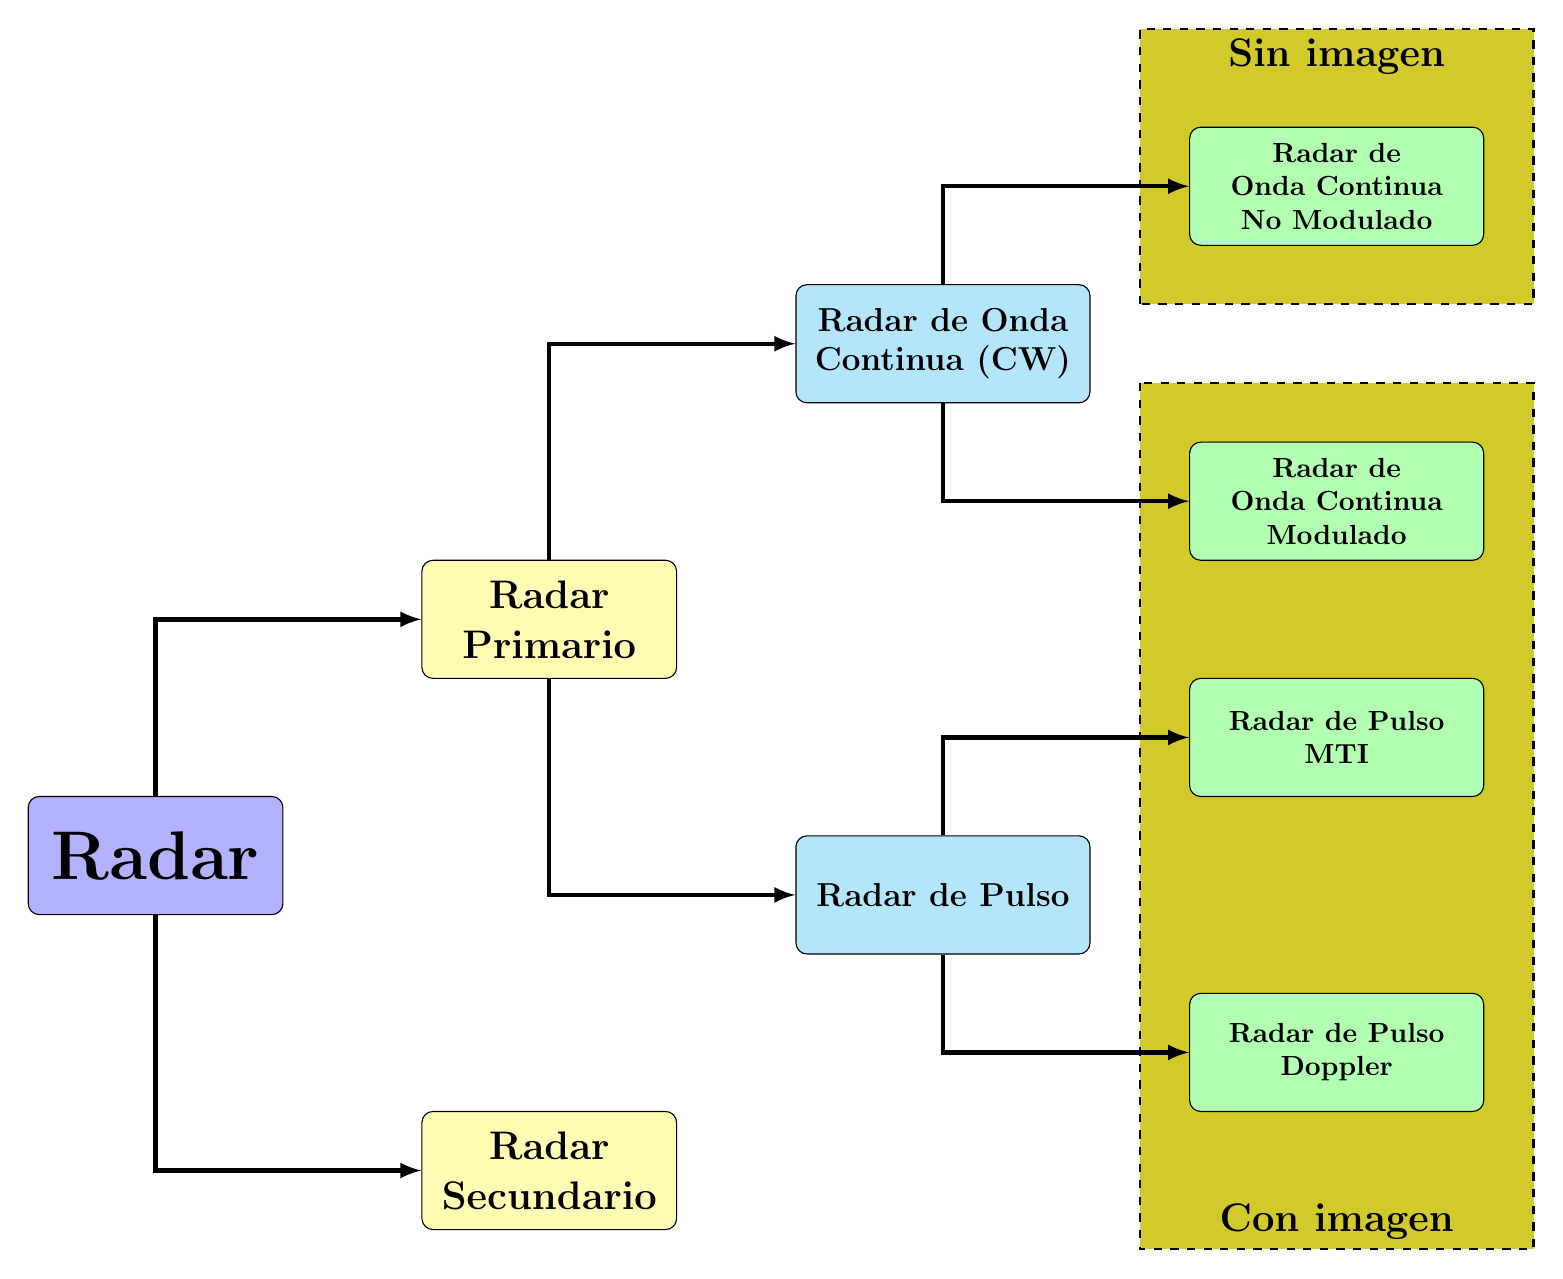
\begin{tikzpicture}[
                node distance = 2cm ,
                every node/.style={
                                       font =  \bfseries , 
                                      } ,
                  NodoPrimario/.style = {
rectangle , draw , rounded corners , 
text centered ,                                         
minimum width = 3cm ,
                                        minimum height= 1.5 cm ,
                                  text width= 3cm ,                     
                                  font = \Large \bfseries ,
                                  fill = blue!30 ,
                                    }  ,
                  NodoSecundario/.style = {
rectangle , draw , rounded corners , 
text centered ,                                         
minimum width = 3cm ,
                                        minimum height= 1.5 cm ,
                                  text width= 3cm ,                     
                                  font = \Large \bfseries ,
                                  fill = yellow!30 ,
                                    }  ,
NodoTerciario/.style = {
rectangle , draw , rounded corners , 
text centered ,                                         
minimum width = 3cm ,
                                        minimum height= 1.5 cm ,
                                  text width= 3.5 cm ,        
                                  font = \large \bfseries ,             
                                  fill = cyan!30 ,
                                  } ,
NodoCuarto/.style = {
rectangle , draw , rounded corners , 
text centered ,                                         
minimum width = 3cm ,
                                        minimum height= 1.5 cm ,
                                  text width= 3.5 cm ,  
                                  fill = green!30 ,
                                  } ,
                ]

% \draw [ green!70!black  , step = 1 cm ] ( 0 , -5 ) grid ( 20 , 10 ) ; 

\draw [ thick , dashed , fill = yellow!80!black ] ( 12.5 , 7.0 ) rectangle  ( 17.5 , 10.5 ) ; 

\node  at  ( 15.0 , 10.15 ) { \Large Sin imagen}  ;

\draw [ thick , dashed , fill = yellow!80!black ] ( 12.5 , 6.0 ) rectangle  ( 17.5 , -5 ) ; 

\node  at  ( 15.0 , -4.65 ) { \Large Con imagen}  ;

\node [ NodoPrimario ]  (radar) { \Huge Radar}  ;

\node [fill = yellow!50 , right of = radar , 
               xshift= 3 cm , yshift = 3 cm  ,                
              NodoSecundario  ] (PSR) {  Radar Primario } ; 

\node [ right of = PSR , 
               xshift= 3 cm , yshift = 3.5 cm  , 
               fill = cyan!30 , 
               NodoTerciario  ] (cw)   {Radar de Onda Continua (CW)	}   ; 

\node [ right of = cw , 
               xshift= 3 cm , yshift = 2 cm  , 
               NodoCuarto  ] (cw_NoModulado)   {Radar de \\ Onda Continua \\ No Modulado	}   ; 

\node [ right of = cw , 
               xshift= 3 cm , yshift = - 2 cm  , 
               NodoCuarto  ] (cw_Modulado)   {Radar de \\ Onda Continua \\ Modulado	}   ; 


\node [ right of = PSR , 
               xshift= 3 cm , yshift = -3.5 cm  , 
               fill = cyan!30 , 
               NodoTerciario  ] (PS)   {Radar de Pulso 	}   ; 

\node [ right of = PS , 
               xshift= 3 cm , yshift = 2 cm  , 
               NodoCuarto  ] (ps_mti)   {Radar de Pulso  \\ MTI	}   ; 

\node [ right of = PS , 
               xshift= 3 cm , yshift = - 2 cm  , 
               NodoCuarto  ] (ps_doppler)   {Radar de Pulso \\ Doppler	}   ; 



\node [fill = yellow!50 , right of = radar ,  
                                 xshift= 3 cm , yshift = -4 cm  ,
                                  NodoSecundario  ] (SSR) { \Large Radar Secundario } ; 


\draw [ ultra thick , -latex ] (radar) |- (PSR) ; 
\draw [ ultra thick , -latex ] (radar) |- (SSR) ; 

\draw [ ultra thick , -latex ] (PSR)	 |- (cw) ; 
\draw [ ultra thick , -latex ] (PSR)	 |- (PS) ; 

\draw [ ultra thick , -latex ] (cw) |- (cw_NoModulado) ; 
\draw [ ultra thick , -latex ] (cw) |- (cw_Modulado) ; 

\draw [ ultra thick , -latex ] (PS) |- (ps_mti) ; 
\draw [ ultra thick , -latex ] (PS) |- (ps_doppler) ; 

\end{tikzpicture}